\section{Control System}\label{sec:sailor}
\subsection{Objectives}
This section describes the design of a controller that is capable of robustly
steering a sailboat along a predefined course while always setting the sail to
the optimal angle to the wind in order to generate as much driving force as
possible. For that, it also has to be able to conduct manoeuvres such as tack
and jibe. At the same time, the controller should take into account the
changing environmental conditions, such as wind speed and direction and react
accordingly. Furthermore, since the path planner (section \ref{sec:navigator})
calculates a global trajectory and relies on the control system to follow this
course, the control system has to compensate for drift.
%
\subsection{Existing Works}
There are various systems available that assist a sailor in steering a
sailboat. Most of these are commercially available autopilots, that operate
either with a built in magnetic compass or with a wind vane
\cite{hochseeportverband1958s}. These systems are finished products, that have
been used for many years and are very robust and reliable. We did not use
commercial products, mainly because of interfacing issues. Autopilots are
designed for a human sailor on board who does the navigation and has to tune
the sails. Although some of the systems are even able to perform tacks and
jibes, the manoeuvre has to be confirmed by the human sailor pressing a button
on the autopilot's control panel. Since the software integrated in commercial
autopilots is typically closed source, this problem cannot be solved by simply
reprogramming the device. Furthermore, most autopilots only control the rudder,
so we would still have to figure out a way to tune the sail.

Apart from the commercial products, there are also several scientific works
regarding control systems for autonomous sailboats, most of them also by
participants in the \textsc{Microtransat}. Developments reach from a fuzzy
logic controller for both rudder and sail \cite{stelzerFuzzy}, over an LQG
controller based on a non-linear 3 degrees of freedom (DOF) model
\cite{elkaim:ska}, up to a complex self learning AI system that has been
successfully tested on an Open60 racing yacht. Our work is mainly influenced by
Briere \cite{briere2008iar}, who describes a simple controller based on a state
machine.
%
\subsection{System Modelling} In order to design a robust controller and
identify parameters in a controlled environment, a simulator is very helpful.
Although there are several sailing simulators available, most of them are made
for gaming. Rather than having an interface that allows them to be steered by a
self-developed control system, they are meant to be operated by hand. For this
reason we implemented a simulator in Matlab/Simulink.

To gain a general system that could later be extended with boat/wave
interaction, the boat was modelled as a rigid body with full 6 DOF. The system
has 12 state variables: 3 for position, 3 for attitude, 3 for velocity and 3 for
turning rates.  Inputs to the plant are rudder angle
$\gamma_{\text{rudder}}$, sail angle $\gamma_{\text{sail}}$, true wind speed
$v_{\text{wind}\_\text{true}}$ and direction $\Psi_{\text{wind}}$, while
outputs are the boat's position and attitude and their corresponding
derivatives.

Forces were introduced at various points of the boat to model the interactions
between water and hull as well as wind and sail.
% \subsubsection{Gravity}
% The only static force acting on our sailing boat is gravity.
\subsubsection{Sail Force}
In order to calculate the force generated by the sail, the apparent wind angle is needed which is computed in a vector operation from the true wind angle and the boat's velocity. The 2 components of the sail force $F_{sail}$ are then modelled using the standard approximation for air foils in a moving fluid
\begin{equation} \label{eqn:air_foil_lift_drag}
\begin{array}{l}
  F_{\text{sail}\_\text{lift}} = \dfrac{1}{2}\cdot \rho_{\text{air}} \cdot v_{\text{wind}\_\text{app}}^2 \cdot A_{\text{sail}} \cdot c_l(\alpha_{\text{sail}})\\
\\
  F_{\text{sail}\_\text{drag}} = \dfrac{1}{2}\cdot \rho_{\text{air}} \cdot v_{\text{wind}\_\text{app}}^2 \cdot A_{\text{sail}} \cdot c_d(\alpha_{\text{sail}})
\end{array}
\end{equation}
where $\rho_{\text{air}}$ is the density of air, $A_{\text{sail}}$ is the
apparent area of the sail and $c_l$ is the lift coefficient which depends on
the sail's shape and the angle of attack $\alpha_{\text{sail}}$.
\subsubsection{Rudder Force}
The rudder force is also modelled using equation \ref{eqn:air_foil_lift_drag},
just with different parameters. Since the rudders are at the stern of the
boat, the force induces a moment around the vertical axis and thus affects the
boat's heading.
\subsubsection{Resistances}
There are several damping forces that depend on the velocity and rate of turn
of the boat. Those are mainly the resistance of hull and keel in all 3 axes of
translational freedom and the damping of rotations. These are modelled using
the equation
\begin{equation}
  F = d \cdot v^2
\end{equation}
where $v$ is the velocity or rate of turn and $d$ is a parameter that has to be
identified in experiments.

After the first tests with the real boat, we found the real boat behaviour to
be quite different from the simulation. To improve this, more tests and
parameter identification needs to be done. Due to time constraints this has not
been done at the time of this writing.

\subsection{Controller Principle}
In our control system layout, rudder and sail are controlled in two separate
Single Input Single Output (SISO) systems that are assumed to be independent of
each other. During testing, this assumption has proved to be very reasonable.

\subsubsection{Sail Control}
For the sail, the controlled value is the angle of attack. This directly
depends on the sail's angle. Since \textsc{Avalon}'s sail and rudder motors
already come with a built in positioning controller, this subsystem is
sufficiently controlled by just writing a reference value to the motor
controller.

This reference value is derived from a predefined optimal Angle Of Attack (AOA)
that was found in experiments. However, for safety reasons, the wanted AOA also
changes dynamically depending on the wind speed. Basically, as the wind speed
increases, the wanted AOA approaches zero, which reduces the sail force
generated by the wind. With this behaviour, the boat remains steerable even in
strong winds.

\subsubsection{Rudder Control}
The second subsystem controls the boat's heading using the rudder as input.
Since the heading changes dynamically and is not directly dependent on the
rudder angle, this system takes a little more consideration. For this purpose,
a heading error minimising PID controller was designed in an iterative process using the Matlab
simulation. It was then tested and optimised in the real boat (see section
\ref{sec:sailor_testing}).

In order to compensate for leeway drift, the boat has to sail somewhat closer
to the wind than the desired heading $DH_{\text{nav}}$ calculated by the path
planner.
Since drift changes considerably with the wind and wave conditions, it is
important to know the current drift in order to compensate for it. \textsc{Avalon}
is equipped with an Inertial Measurement Unit (IMU) with a built in GPS
receiver. With this sensor, the drift speed $v_{\text{drift}}$ can be accurately
measured at any time. From the drift, a new desired heading DH$_{\text{sailor}}$ is
calculated using the equation
\begin{equation}
  \text{DH}_{\text{sailor}} = \text{DH}_{\text{nav}} + \arctan\left( \frac{v_{\text{drift}}}{v_{\text{boat}}} \right)
\end{equation}

\subsubsection{State Machine}
A sailboat can not sail at all angles to the wind. Figure \ref{fig:courses_to_wind} shows the ranges that we cannot sail in gray. In order to sail as fast as possible, it has to be differentiated between different types of sailing. To this end, the controller is designed as a state machine that switches states depending on the angle to the wind. The 5 states are depicted in figure \ref{fig:courses_to_wind}.
\begin{figure}[htb]
\centering
% trim = left bottom right top
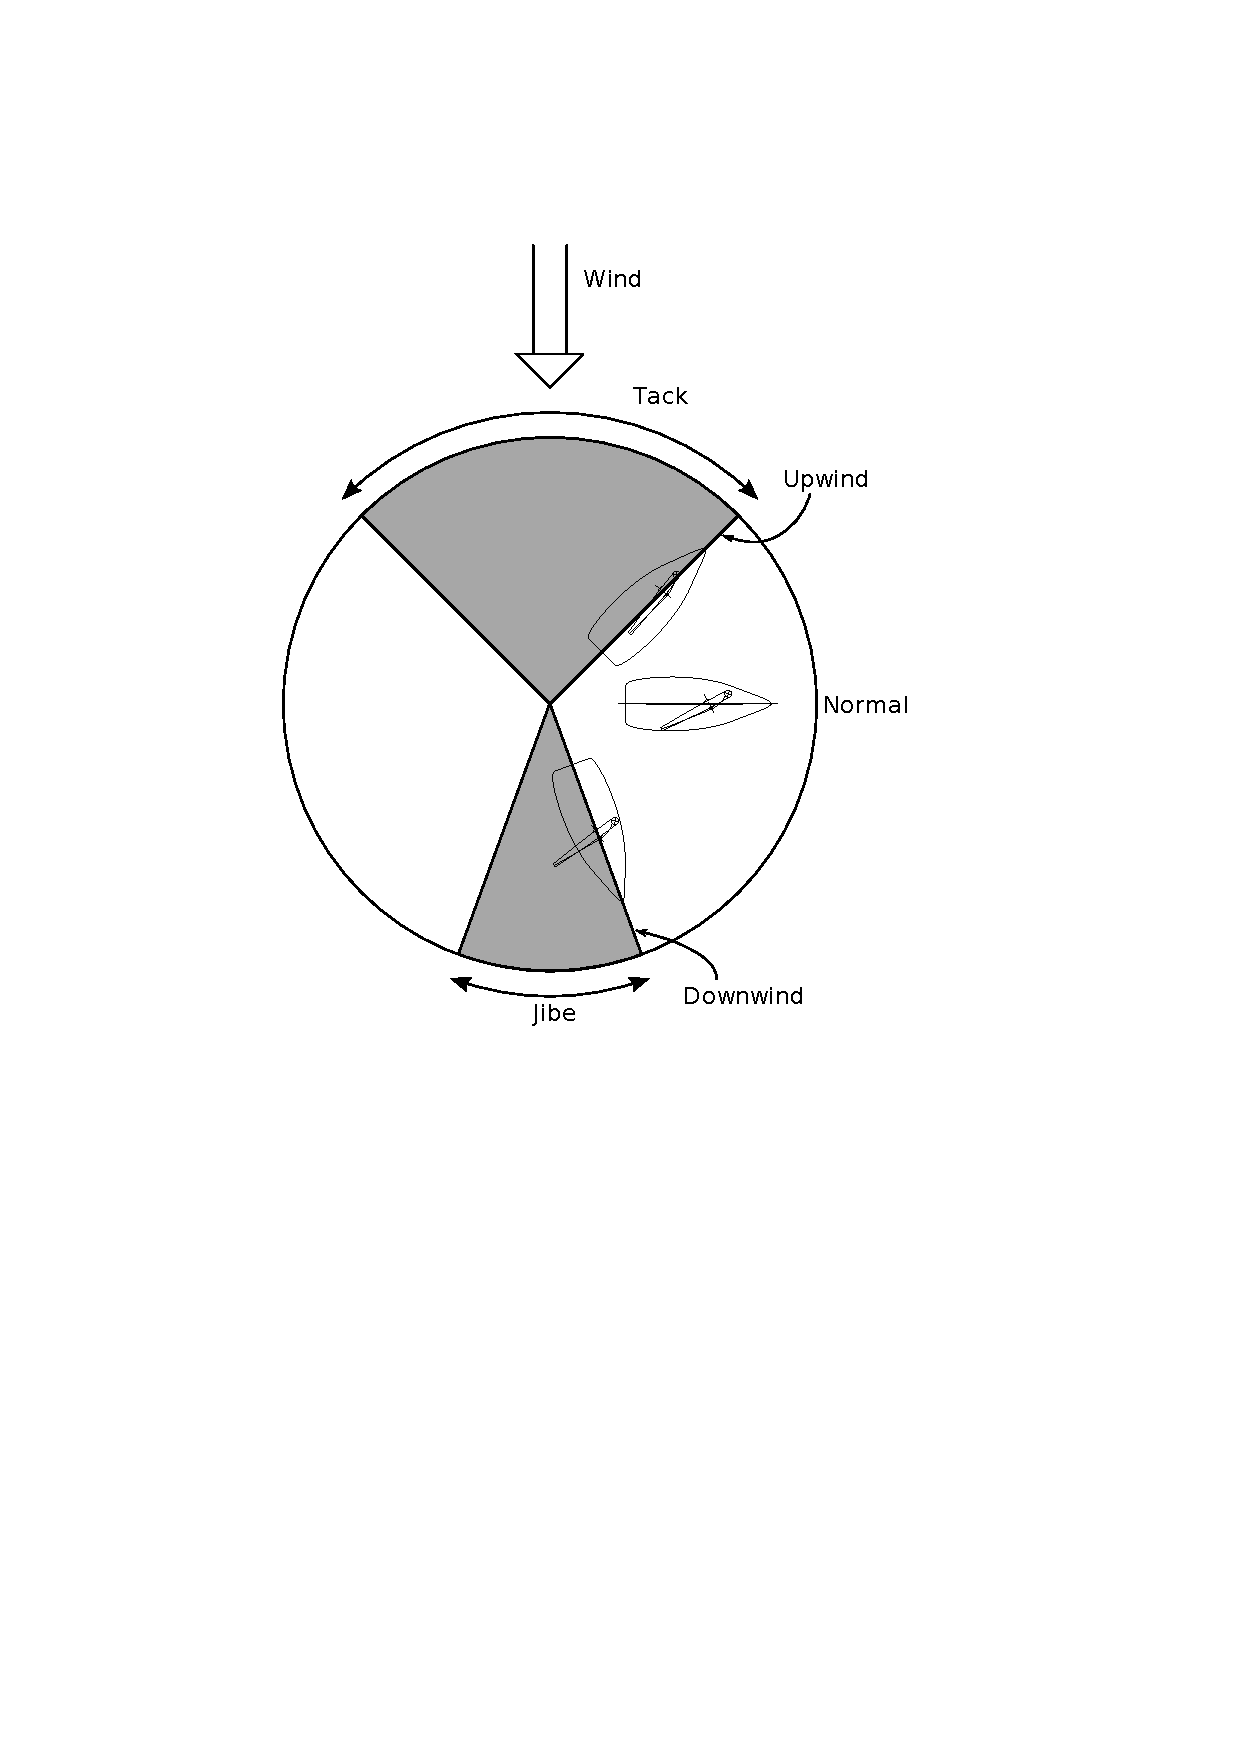
\includegraphics[trim = 45mm 120mm 55mm 45mm, clip, width=0.70\columnwidth]{pics/courses_to_wind.pdf}
\caption{Possible courses of a sailing yacht with respect to the wind and corresponding control system states. The range with wind directly from behind could be sailed in theory, but is not very efficient and rather unstable.}\label{fig:courses_to_wind}
\end{figure}
\subsubsection{Normal Sailing}
If the desired heading given by the path planner (section \ref{sec:navigator}) is
in the sailable (white) range, the system is in state \texttt{Normal Sailing}.
In this state the rudder controller follows the given desired heading, while
the sail controller permanently adjusts the sail to achieve the optimal angle
of attack on the sail. If the desired heading changes within the sailable
range, the rudder controller simply follows the new course while the sail
controller maintains a constant angle of attack.
\subsubsection{Upwind Sailing}
If the desired heading for whatever reason is set in the not sailable (gray)
range, it cannot be directly followed. The objective in this case is to make as
much velocity towards the wind as possible. In \texttt{Upwind Sailing} mode the
sail is set to the tightest position that is reasonably possible. While the
sail angle is kept at this constant position, the rudder controller now keeps a
constant heading angle to the true wind and thus takes advantage of all wind shifts.
Note that the behaviour is similar for downwind sailing.
%
\subsection{Test Results and Analysis} \label{sec:sailor_testing}
Several tests were undertaken to verify and optimise the control system. Before
any testing on the water was done, the state machine's transition conditions
had to be verified. This was done by putting the boat on a trailer on a
sufficiently windy day and turning it around its vertical axis while constantly
checking the current state. We encountered many problems that were caused by
the sign change between $-180^o$ and $+180^o$. Some time could have been saved,
if the whole control program, including the state machine, had been tested more
thoroughly in the simulation environment.

The controller was then tested for its ability to keep a desired heading and to
react to changes in desired heading. After some tuning of the PID parameters we
found that the parameters in table \ref{tab:pid_params} yield fast reactions
without too much overshoot.
%
\begin{table}[htb]
\caption{PID Parameters} \label{tab:pid_params}
\centering
\begin{tabular}{c|l}\hline
P & 0.3  \\ \hline
I & 0.005 \\ \hline
D & 30 \\ \hline
\end{tabular}
\end{table}
%
A step response in winds of about 20 knots is illustrated in figure
\ref{fig:step_response_wind20kn}. Note that 20 knots is already a strong wind
and that in lower wind speeds we experienced much less oscillation around the
reference value. Even this $\pm 10^o$ oscillation that is mostly caused by
waves can barely be seen on the boat. We then also applied disturbances to the
boat by deviating it from its course by hand. The reaction was the same as with
changes in desired heading.
%
\begin{figure}[thb]
\centering
% trim = left bottom right top
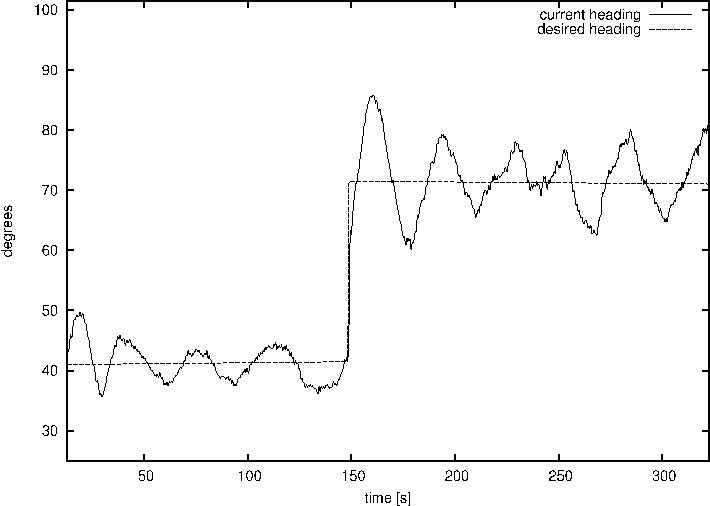
\includegraphics[trim = 0mm 0mm 0mm 0mm, clip, width=7cm]{pics/reference_step_usee4_2.pdf}
\caption{Step response in state \texttt{Normal Sailing}. Conditions were 20\,kn wind from 140°}\label{fig:step_response_wind20kn}
\end{figure}

Figure \ref{fig:3tacks_upwind_sailing} shows current heading, desired heading
and wind direction during three tacks. Between the tacks, the controller state
machine is in state \texttt{Upwind Sailing}. It can be very well seen, that the
boat keeps a constant angle to the wind and takes advantage of wind shifts as
expected.
\begin{figure}[thb]
\centering
% trim = left bottom right top
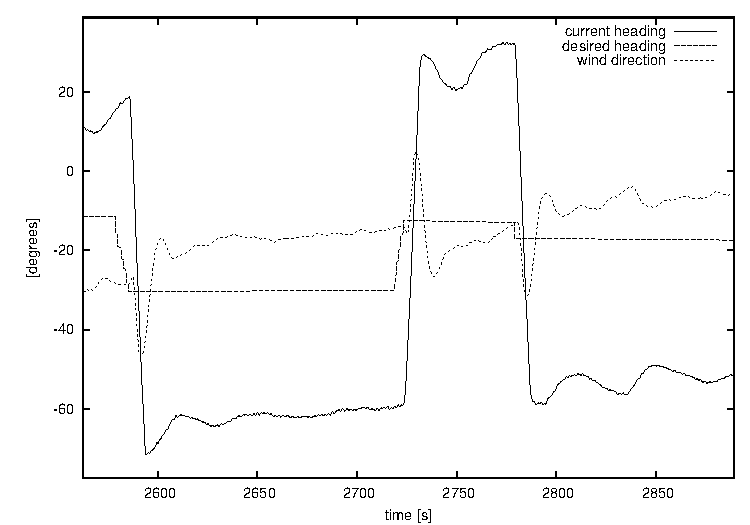
\includegraphics[trim = 0mm 0mm 0mm 0mm, clip, width=7cm]{pics/tacks_to_upwind_usee5_wind8kn_hdg.pdf}
\caption{3 tacks, with \texttt{Upwind Sailing} in between.}\label{fig:3tacks_upwind_sailing}
\end{figure}
A lot of time was invested into correct timing during tack and jibe. In the
beginning we had several problems that resulted in inappropriate sail tuning
during or right after manoeuvres. This sometimes even resulted in the boat
sailing backwards.

Figure \ref{fig:wyp_autonom_drift_comp} shows how the boat follows a trajectory
that was calculated by the path planner. The path planner's calculation was started
at the bottom left where the dashed line begins. After the calculation was
completed, the boat jibes and sets the new course. After a few seconds the
drift compensation starts to work and the boat's real course approaches the
desired trajectory.
%
\begin{figure}[thb]
\centering
% trim = left bottom right top
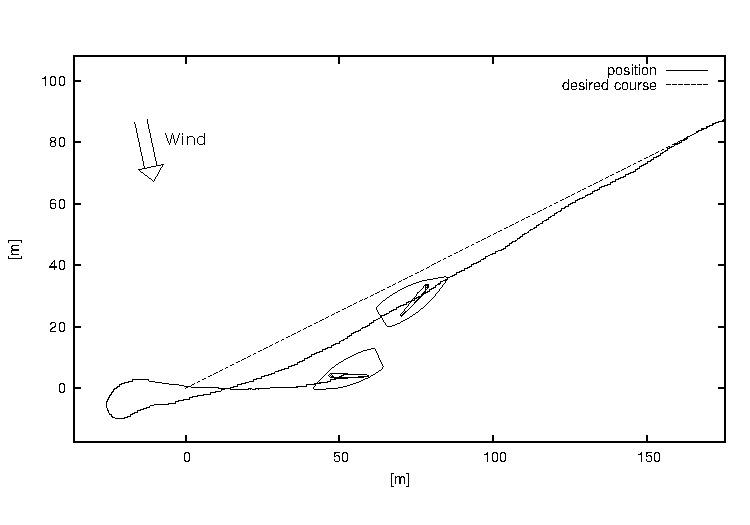
\includegraphics[trim = 0mm 0mm 0mm 0mm, clip, width=7cm]{pics/driftcompensation.pdf}
\caption{GPS plot of the controller following a desired trajectory calculated
by the path planner. It was recorded during a test on the Urnersee in about 15
knots wind.}\label{fig:wyp_autonom_drift_comp}
\end{figure}

